\section{Introduction}
\label{sec:intro}
Slang terms are widely used in social media and novel slang terms emerge all the time, but understanding such slang terms across languages can be a very challenging task.
Consider the following question:
 {\em What are the English terms that can help us understand the meaning of the Chinese slang term``浮云''? \footnote{{\scriptsize ``浮云'' is a Chinese slang term, which literally means ``floating clouds''. However,  it almost always means something as ephemeral and unimportant as ``passing clouds'', both on the Internet and in everyday life.}}} 
We find that both existing dictionaries and state-of-the-art machine translators often just translate such slang terms to their literal meanings, 
even under a clear context where slang meanings are much more appropriate.  

Given a slang term in one language, our research problem is to find terms in another language which can help people understand its meaning.
We believe this research area not only can assist people to communicate better in cross-cultural situations but also improves the performance of existing machine translation systems.  
Attacking this research problem, we make the following contributions in this paper:
\begin{enumerate}
	\itemsep0em 
	\item To the best of our knowledge, we are the first to propose a task about understanding slang cross-lingually. 
	We also provide a benchmark dataset for evaluation which can benefit  further research in this area. 
	
	\item We propose a straightforward but effective approach to build bilingual word representations (\textit{\socvec}) from social media. 
	With \textit{\socvec}, we can simply compute cross-lingual word similarities to find target terms. 
	\item Qualitative and quantitative evaluation  show that our proposed approach outperforms the baseline methods.
\end{enumerate}
%\vspace{-10pt}
\section{Dataset Building and Task Description}
%\vspace{-10pt}
We first introduce how we build our dataset for the proposed task.\footnote{{\scriptsize Due to the salient cross-cultural differences between the east and the west, we choose English and Chinese as the example language pair in this paper.}} 
We use an online Chinese slang glossary\footnote{\tiny{\url{https://www.chinasmack.com/glossary}}} consisting of  200 popular slang terms with English explanations to construct the ground truth target English terms by extracting most related words.  
%For each Chinese slang term, we extract the ground truth target English terms from its explanation in the glossary, which can help people understand their slang meanings.  
For example, we extract the most relevant words (boldfaced) in the glossary entry of the Chinese slang term ``二百五'' as follows:
\begin{description}
%	\vspace{-10pt}
	\item[二百五]: A \textbf{\textit{foolish}} person who is lacking in sense but still \textbf{\textit{stubborn}}, \textbf{\textit{rude}}, and \textbf{\textit{impetuous}}.
\end{description}
Similarly for English slang terms, we resort to a slang word list from OnlineSlangDictionary\footnote{\tiny{\url{http://onlineslangdictionary.com/word-list/}}} with translated explanations and then down-sample the list to 200 terms as well.  
%Similarly, for each English slang term of interest, we extract the important words from its explanation and then utilize their translations as the final ground truth.
%
%Different methods should produce a list of translation terms 
%as similar as possible to the ground truth target terms.
%Finally, for each English or Chinese slang term, we have a set of target Chinese or English terms which are considered to be helpful for understanding slang across languages.

Given any slang term in a \textit{source} language in this dataset, our proposed task is to find a set of words in another \textit{target} language that should be close to the ground truth word set. 
\vspace{-5pt}
\section{Baseline Methods}
We propose two types of baseline methods for this task. 
The first type is based on well-known {\em on-line translators}, 
namely Google, 
Bing and Baidu.  
%With our test set's slang as input, we retrieve the output of translation. 
A specific baseline method for Chinese slang is from CC-CEDICT\footnote{{\scriptsize An on-line public-domain Chinese-English dictionary, which is well updated with popular slang terms. \url{https://cc-cedict.org/wiki/}}} (CC).
%Considering situations that many slang terms have literal meaning, it is unfair to retrieve target terms from such on-line translators by simply inputing slang terms without slang contexts. 
%We use example sentences with slang terms from some websites (mainly from Urban 
%Dictionary\footnote{\scriptsize{\url{http://www.urbandictionary.com/}}}) 
%as input for such translators, so that they are expected to have a great chance of knowing this is
%a slang use. 
%\footnote{Nevertheless, we noticed
%	that the on-line translators often ignore the slang contexts and still produce
%	literal translations.}
%The following example shows how we obtain the target translation terms 
%for the slang word ``fruitcake'' (an insane person) from Google Translator:

%\noindent
%\textit{Input Sentence:}
%{\textit{Oh man, you don't want to date that girl. She's always drunk and yelling. She is a total \underline{fruitcake}.}}\footnote{{\url{http://www.englishbaby.com/lessons/4349/slang/fruitcake}}}\\ 
%\textit{Google Translation:}
%{\small哦, 男人, 你不想约会那个女孩。她总是喝醉了, 大喊大叫。她是一个\underline{水果蛋糕}。}

The second type of baseline methods are ranking based. 
We score each of the possible term in the target language and consider the top five as the target 
terms. 
%Given a source term to be translated, several such {\em ranking-based 
%	baseline methods} are as follows.
Existing \textit{cross-lingual word representation} models can be applied to compute the semantic similarities of terms across languages.
Thus, we score all candidate target terms by computing cosine similarities in their constructed bilingual vector spaces with different models: Linear Transform (LT)~\cite{Mikolov:2013tp}, MultiCCA, MultiCluster~\cite{ammar2016massively} and Duong~\cite{DBLP:conf/emnlp/DuongKMBC16} methods. 
A more sophisticated baseline method, TransBL, first translates each candidate target term back into the source language with a bilingual dictionary. Then, we calculate the average cosine similarities between the source term and the translated terms in monolingual word vector space as the scores to rank. 
\vspace{-10pt}
\section{\socvec ~Model}
\begin{figure}[]
	\centering
	\caption{Workflow for computing the cross-cultural similarity between 
		an English word \textit{W} and a Chinese word \textit{U}.}
	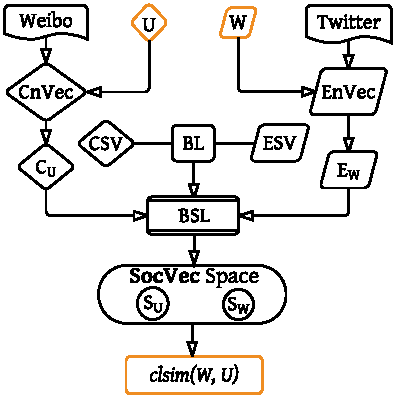
\epsfig{file=figures/overview.pdf, width=0.5\columnwidth}
	
	\label{fig:overview}
	\vspace{-10pt}
\end{figure}
In this paper, we propose a novel approach to project 
two heterogeneous monolingual word vector spaces into 
one bilingual word vector space, known as 
social vector space (\textit{\socvec}), 
by constructing a bilingual social lexicon (BSL) consisting of bilingual mappings of selected \textit{social word}s
that reflect opinion, sentiment, cognition and many other psychological 
processes. 
These words, we believe, are central to capturing cultural semantics.
%using only a bilingual lexicon (for common words), two monolingual socio-linguistic vocabularies and a comparable corpus\footnote{A comparable corpus is a pair of corpora in two different languages, which come from the same domain.} from microblogs, all of which are easily available.

Each dimension of our \textit{\socvec}~then represents a \textit{socio-linguistic} feature 
derived from mono-lingual semantic similarities between an input term and 
each corresponding entry in the BSL. 
Consequently, a term $W$ in language $L_1$ and a term $U$ in 
language $L_2$ can each be respectively projected 
into a bilingual word vector in the \textit{\socvec} while maintaining
their social features. Thus, cross-cultural similarities can be computed directly with vectors from \textit{SocVec}. 

\figref{fig:overview} shows the overall workflow of our approach to construct the \textit{SocVec} and compute cross-lingual similarity between $W$ and $U$, denoted as $\text{clsim}(W,U)$. 
\footnote{{\scriptsize Notations are as follows: CnVec = Chinese word vector space, EnVec = English word vector space, CSV = Chinese social word vocab, ESV = English social word vocab, BL = Bilingual Lexicon, BSL = Bilingual Social Lexicon.
Finally, $\mathbf{E_x}$, $\mathbf{C_x}$ and $\mathbf{S_x}$ are the word vectors of word $x$ (either $U$ or $W$) in EnVec space, CnVec space and SocVec space respectively.}} 
With such cross-lingual similarities, we can easily compute the score of each candidate target terms like other ranking-based baseline methods explored above.       
%Thanks to the large size of our social word vocabulary and the developing process,(around 3k-5k)  
%Note that \textit{ScoVec} is an encoding for words across languages, where each dimension has 
%clear meaning.
\section{Evaluation}
We first show two 
examples of translations of different methods for qualitative evaluation:
% && Water army& Navy& Navy & propaganda, complicit, fraudulent
\begin{description}
	%	\vspace{-10pt}
	\item[1) 水军] This slang term literally means ``water army'', but its slang meaning is the people paid to slander competitors on the Internet and to help shape public opinion. The results of Google, Bing and Baidu translators are \textbf{``\textit{Water} \textit{Navy}''}, which is the literal meaning of this slang term. However, our \textit{\socvec}  can produce words such as \textbf{{``\textit{propaganda}'', ``\textit{complicit}'', ``\textit{fraudulent}''}}, reflecting its real slang meanings.
	
	\item[2) fruitcake] This slang term means a crazy person, or someone who is completely insane. 
	We found that all online translators treat it as ``\textit{\textbf{fruit cake}}'', even given a context like ``\textit{She’s always drunk and yelling, and she is a total fruitcake.}''\footnote{{\tiny \url{ http://www.englishbaby.com/lessons/4349/
slang/fruitcake}}}. 
	In contrast, our method can capture the slang meaning and produce words like \textbf{``厌烦''{\textit{(annoying)}}, ``疯狂''\textit{(crazy)} } and \textbf{ ``怪诞''\textit{(bizarre)}.}
\end{description} 
% 
%Our results are highly correlated with these explanations and capture their core semantics, whereas most online translators just offer literal translation of such slang terms, even with the ample slang contexts.

To quantitatively evaluate different methods, we need to measure similarities between the produced target term sets and the ground truth word sets.
Exact-matching based similarity is too strict to capture valuable relatedness between two word sets.  
We argue that the\textit{ Average Cosine Similarity} (ACS) between two sets of word vectors is a better metric to evaluate the similarity between two word sets:
\begin{align*}
\vspace{-3pt}
ACS (A,B)=
{\frac{1}{|A||B|}}{\sum_{i=1}^{|A|}{\sum_{j=1}^{|B|}} \frac{\mathbf{A_i }\cdot \mathbf{B_j}}{\|\mathbf{A_i }\|\|\mathbf{B_j }\|}}
\vspace{-2pt}
\end{align*} 
where $A$ and $B$ are the two word sets; $\mathbf{A_i}$ and $\mathbf{B_j}$ are the two word vectors of the $i^{th}$ word in $A$ and $j^{th}$ in $B$ respectively\footnote{{\scriptsize The word vectors used in ACS computation is a third-party pre-trained 
		embedding and thus ACS computation is fair over different methods.}}. 
\tabref{tab:bleis_acs} shows the quantitative evaluation results. 
\begin{table}[] 
	\caption{ACS Sum Results of Slang Translation 	\vspace{-10pt}}
	\small
	\centering
	\begin{subtable}[h]{0.9\columnwidth}
		\centering
		\begin{tabular}{|ccccc|}
			\hline
			Google&  Bing& Baidu & CC & LT   \\ 
			18.24 &  16.38&  17.11 & 17.38 & 9.14 \\ \hline
			TransBL& MultiCCA & MultiCluster & Duong   & \textbf{\socvec} \\ 
			18.13 &  17.29 & 17.47&  20.92& \textbf{23.01}\\ \hline  
		\end{tabular}
		\subcaption{Chinese Slang to English}
	\end{subtable}
	\begin{subtable}[h]{0.9\columnwidth}
		\centering
		\begin{tabular}{|ccccc|}
			\hline
			Google&  Bing& Baidu &  LT   & TransBL\\ 
			6.40  &   15.96 &  15.44  & 7.32 & 11.43\\    \hline
			MultiCCA & MultiCluster & Duong   & \textbf{\socvec} & \\ 
			15.29 & 14.97&  15.13& \textbf{17.31} & \\ \hline  
		\end{tabular}
		\subcaption{English Slang to Chinese}
	\end{subtable}
	
	\label{tab:bleis_acs}
\end{table}

\vspace{-5pt}
\section{Conclusion and Future Work} 
We propose a novel task about understanding slang across languages with a benchmark data set. Also, experiments show that our proposed \socvec~ based method is more effective than other strong baseline methods. 
Future directions include further development of larger datasets for more languages and then proposing supervised methods.

